\documentclass[11pt, a4paper]{report}

% ===== ENCODING & LANGUAGE =====
\usepackage[utf8]{inputenc}
\usepackage[T1]{fontenc}
\usepackage[english]{babel}
\usepackage{textcomp}
\usepackage{newtxtext}

% ===== PAGE LAYOUT =====
\usepackage[paperwidth=8.5in,paperheight=11.0in,left=1.125in,right=0.875in,top=0.875in,bottom=0.875in]{geometry}
\usepackage{setspace}
\onehalfspacing

% ===== TEXT ALIGNMENT =====
\usepackage{ragged2e}
\justifying

% ===== GRAPHICS & FIGURES =====
\usepackage{graphicx}
\graphicspath{{./images/}{./}}
\usepackage{float}
\usepackage{caption}

% ===== TABLES =====
\usepackage{longtable}
\usepackage{multirow,booktabs}
\usepackage{array}

% ===== MATH =====
\usepackage{amsmath}
\usepackage{amssymb}

% ===== UNITS =====
\usepackage{siunitx}

% ===== TIKZ =====
\usepackage{tikz}
\usetikzlibrary{shapes.geometric, arrows, arrows.meta, positioning, chains,
                decorations.pathreplacing, shadows.blur}

% ===== CODE LISTINGS =====
\usepackage{listings}
\usepackage{xcolor}
\lstset{
    language=C,
    basicstyle=\ttfamily\small,
    keywordstyle=\color{blue},
    commentstyle=\color{gray},
    stringstyle=\color{red},
    breaklines=true,
    showstringspaces=false,
    tabsize=4,
    numbers=left,
    numberstyle=\tiny\color{gray},
    frame=single
}

% ===== CITATIONS & REFERENCES =====
\usepackage{cite}
\usepackage[hidelinks]{hyperref}

% ===== FORMATTING =====
\usepackage{color}
\usepackage{titlesec}
\usepackage{enumitem}

% ===== CHAPTER FORMATTING =====
\titleformat{\chapter}[display]
  {\normalfont\bfseries\Huge}
  {\chaptertitlename\ \thechapter}{20pt}{\Huge}
\titlespacing*{\chapter}{0pt}{0pt}{40pt}

% ===== NO PARAGRAPH INDENTATION =====
\setlength{\parindent}{0pt}
\setlength{\parskip}{1em}

\begin{document}
\setlength{\parindent}{0pt}
\setlength{\parskip}{2ex plus 0.5ex minus 0.2ex}
\linespread{1.2}
\tolerance2000

\pagestyle{empty}

%--------------------------------------------------------------
% TITLE PAGE
%--------------------------------------------------------------
\begin{center}
\begin{figure}[H]
    \centering
    
\includegraphics[width=0.55\linewidth]{fig00_biust_logo.png}
\end{figure}
\vspace*{0.5cm}

{\large\Large\textbf{Digital Voting System Using a PIC16F877A Microcontroller}}\\

\vspace*{1.5cm}

{\large
\begin{tabular}{ll}
    Full Name: & Tsotlhe Seiphepi \\
    Student ID: & 21001137 \\[4pt]
    Full Name: & Kgotso Mathangwane \\
    Student ID: & 21000459 \\
\end{tabular}\\[1.2cm]
Module Instructor: Jwaone Gababoitaolelwe \\}

\vspace*{1.0cm}

CTEN 415 --- Microcontrollers \\
Department of Electrical, Computer and Telecommunications Engineering\\
Faculty of Engineering and Technology\\
Botswana International University of Science and Technology\\
Botswana, Palapye

\vspace*{0.6cm}

{\em In partial fulfilment of the requirements for the module CTEN 415}

\vspace*{0.4cm}

{\bf November 2024}

\vfill
\end{center}

\newpage
\clearpage

%--------------------------------------------------------------
% FRONT MATTER
%--------------------------------------------------------------
\newpage
\pagenumbering{roman}
\onehalfspacing
\tableofcontents
\listoffigures
\newpage

%--------------------------------------------------------------
% MAIN CONTENT
%--------------------------------------------------------------
\pagenumbering{arabic}
\onehalfspacing

% ============================================================
\chapter{Introduction}
% ============================================================

This report details the design and implementation of a digital voting system
using a PIC16F877A microcontroller. The system provides a user-friendly and
secure platform for casting votes, with a \(20 \times 4\) LCD to display
candidate information and a \(4 \times 4\) matrix keypad allowing voters to
input their choices.

The system enforces PIN-based authentication before voting begins and again
before vote tallies are displayed, ensuring that sensitive data remains
accessible only to authorised personnel. LED indicators give voters immediate
visual feedback: a red LED blinks three times at start-up and stays on during
operation; a green LED blinks upon a successfully confirmed vote.

\section{Background}

Modern elections demand reliability, accuracy, and tamper resistance.
Embedded microcontroller systems offer a compact, low-cost path to electronic
voting that does not require a networked computer. The PIC16F877A is a
well-documented, widely taught 8-bit microcontroller produced by Microchip
Technology, making it an appropriate platform for a university-level
demonstration of a secure embedded input system.

\section{Objectives}

\begin{itemize}
    \item Develop a digital voting system enabling voters to select candidates
          using a \(4 \times 4\) keypad.
    \item Implement a clear and user-friendly interface on an LCD display.
    \item Ensure accurate and secure vote recording using
          microcontroller-based logic.
    \item Utilise LED indicators to provide visual feedback on voting status.
    \item Incorporate PIN-based security to protect sensitive vote data.
\end{itemize}

% ============================================================
\chapter{Theory}
% ============================================================

\section{Microcontrollers}

A microcontroller (MCU) is a compact computer on a single integrated circuit,
designed to control specific tasks within electronic systems. It integrates a
CPU, memory, and input/output interfaces on one chip. Microcontrollers are
widely used in embedded systems such as home appliances, automotive systems,
medical devices, and consumer electronics \cite{geeksforgeeks}.

A typical microcontroller includes a processor core for executing
instructions, volatile and non-volatile memory for data and program storage,
and I/O peripherals for interacting with the external environment. They also
support various communication interfaces.

Microcontrollers are programmable, allowing customisation for specific tasks.
Common programming languages include C, C++, and assembly language. Designed
for low-power operation, they are ideal for battery-operated devices and are
embedded in a wide range of products, from consumer electronics to industrial
equipment \cite{geeksforgeeks}.

\subsection{Working of a Microcontroller}

The microcontroller chip is a high-speed device but slow compared to a general-purpose
computer. The quartz oscillator is enabled through the control logic register
once the supply is powered on. Parasite capacitors recharge for a few seconds
during early preparation. Once the voltage level reaches its maximum value and
the oscillator frequency stabilises, writing bits through special function
registers becomes stable. Everything is controlled by the oscillator CLK, and
the whole electronics begin to function within nanoseconds \cite{geeksforgeeks}.

\subsection{Microcontroller Properties}

\begin{itemize}
    \item Microcontroller devices are capable of having words longer than 64 bits.
    \item Microcontrollers consist of RAM, ROM, Timer, and I/O Ports.
    \item ROM is used for program storage; RAM is used for data storage.
    \item It is designed using CISC architecture.
    \item Power consumption of modern microcontrollers is significantly lower
          with an operating voltage range from \SI{1.8}{V} to \SI{5.5}{V}.
    \item The latest feature of a microcontroller is flash memory such as
          EPROM and EEPROM \cite{geeksforgeeks}.
\end{itemize}

\section{PIC16F877A Microcontroller}

\subsection{Architecture}

The PIC16F877A is based on the Harvard architecture, which separates memory
space for program instructions and data, allowing efficient and simultaneous
access to both. This enhances the performance of the microcontroller
\cite{microchip}.

\begin{figure}[H]
    \centering
    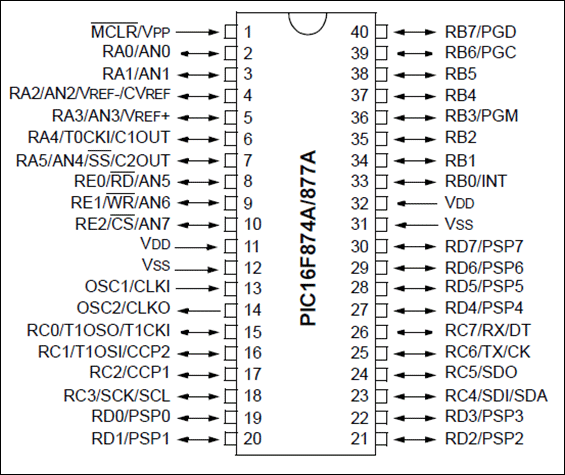
\includegraphics[width=0.65\textwidth]{fig01_pic16f877a_pinout.png}
    \caption{PIC16F877A pinout diagram \cite{microchip}.}
    \label{fig:pinout}
\end{figure}

\subsection{Key Components}

\begin{itemize}
    \item \textbf{CPU:} Executes instructions and controls the flow of data.
    \item \textbf{Memory:} 8\,KB Flash program memory, 368 bytes RAM,
          256 bytes EEPROM.
    \item \textbf{I/O Ports:} 33 configurable pins for digital/analogue input,
          PWM output, or serial communication.
    \item \textbf{Timers:} Used for timing events and generating specific time
          delays.
    \item \textbf{ADC:} 10-bit analogue-to-digital converter on 8 channels.
    \item \textbf{Serial Communication Modules:} UART, SPI, and
          I\textsuperscript{2}C.
    \item \textbf{Interrupt System:} Enables the microcontroller to respond
          to external events efficiently.
\end{itemize}

\subsection{I/O Port Descriptions}

\begin{table}[H]
\centering
\caption{PIC16F877A I/O port summary}
\label{tab:ports}
\begin{tabular}{p{1.5cm}p{1.2cm}p{8.5cm}}
\toprule
\textbf{Port} & \textbf{Width} & \textbf{Description} \\
\midrule
A & 7-bit  & Input or output; direction set by TRISA register. \\
B & 8-bit  & Input or output; four bits respond to interrupt signals in
             input mode. \\
C & 8-bit  & Input or output; direction set by TRISC register. \\
D & 8-bit  & Slave port for microprocessor connection; all pins have
             Schmitt Trigger buffers in I/O mode. \\
E & 3-bit  & Control signals to the A/D converter. \\
\bottomrule
\end{tabular}
\end{table}

\subsection{Supported Communication Protocols}

\begin{itemize}
    \item \textbf{UART} (Universal Asynchronous Receiver-Transmitter): Serial
          communication with other devices.
    \item \textbf{SPI} (Serial Peripheral Interface): High-speed communication
          with sensors, displays, and memory chips.
    \item \textbf{I\textsuperscript{2}C} (Inter-Integrated Circuit):
          Low-speed communication with multiple devices on a single bus.
\end{itemize}

\section{LCD 16$\times$2 Module}

The Liquid Crystal Display (LCD) is a passive device that does not emit light
itself. The \(16 \times 2\) LCD uses a parallel interface requiring multiple
pins to transmit data and control signals. Some variants offer an
I\textsuperscript{2}C interface that reduces pin count \cite{raystar}.

\begin{figure}[H]
    \centering
    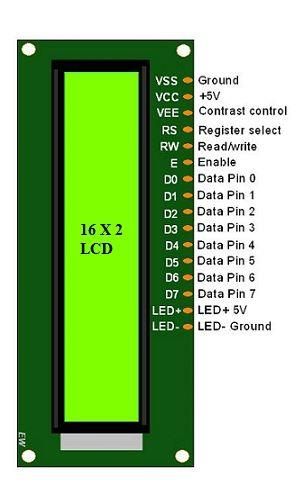
\includegraphics[width=0.55\textwidth]{fig02_lcd16x2_pinout.jpeg}
    \caption{LCD \(16 \times 2\) pinout diagram \cite{raystar}.}
    \label{fig:lcd-pinout}
\end{figure}

The LCD operates using two registers:
\begin{itemize}
    \item \textbf{Command Register:} Stores instructions to control LCD
          behaviour (clear screen, cursor positioning, initialisation).
    \item \textbf{Data Register:} Stores ASCII codes of characters to be
          displayed.
\end{itemize}

\begin{table}[H]
\centering
\caption{LCD module control and data lines}
\label{tab:lcd-pins}
\begin{tabular}{p{2.0cm}p{2.2cm}p{7.0cm}}
\toprule
\textbf{Pin} & \textbf{State} & \textbf{Function} \\
\midrule
EN (Enable) & HIGH pulse & Signals the LCD to latch the data bus. \\
RS (Register Select) & LOW & Data is a command. \\
              & HIGH & Data is a character for display. \\
RW (Read/Write) & LOW & Write to LCD. \\
                & HIGH & Read from LCD. \\
D4--D7 & --- & 4-bit data bus (7 lines total in 4-bit mode). \\
\bottomrule
\end{tabular}
\end{table}

\section{4$\times$4 Matrix Keypad}

A \(4 \times 4\) matrix keypad is a matrix-based input device consisting of
16 buttons arranged in 4 rows and 4 columns, requiring only 8 pins
\cite{elektronicavoorjou}.

\begin{figure}[H]
    \centering
    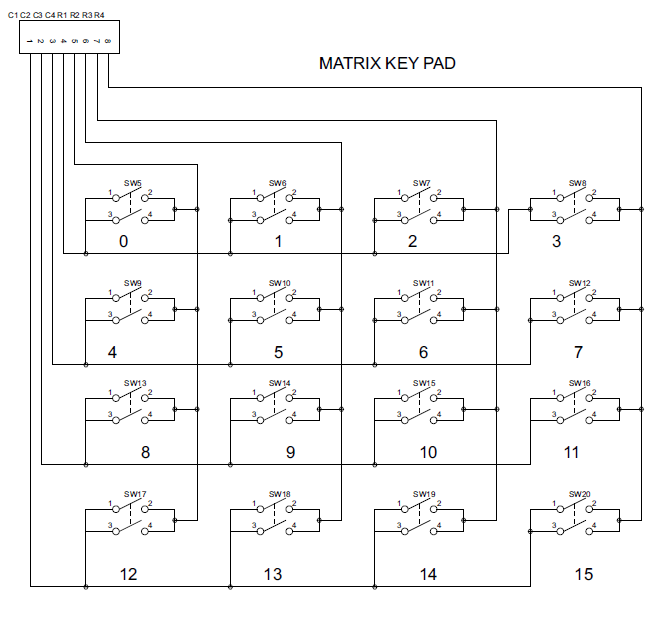
\includegraphics[width=0.60\textwidth]{fig03_matrix_keypad_internal.png}
    \caption{Internal structure of the \(4 \times 4\) matrix keypad
             \cite{lastminuteengineers}.}
    \label{fig:keypad}
\end{figure}

\subsection{Keypad Scanning}

\begin{enumerate}
    \item Each row is connected to an input pin; each column is connected to
          an output pin.
    \item Input pins are pulled HIGH by enabling internal pull-up resistors.
    \item The microcontroller sequentially drives each column pin LOW and
          checks all row pins.
    \item If a row pin reads LOW, the button at that row/column intersection
          is pressed.
    \item The microcontroller waits for release, then looks up the character
          in the keymap array.
\end{enumerate}

% ============================================================
\chapter{Methodology}
% ============================================================

\section{Materials and Software}

\begin{table}[H]
\centering
\caption{Hardware and software used in the project}
\label{tab:materials}
\begin{tabular}{ll}
\toprule
\textbf{Item} & \textbf{Specification / Purpose} \\
\midrule
PIC16F877A & 8-bit microcontroller, main controller \\
20$\times$4 LCD (LM044L) & Display for system messages and candidates \\
4$\times$4 Matrix Keypad & Voter and administrator input \\
Crystal Oscillator & 8\,MHz external clock \\
Capacitors & 2$\times$ 22\,pF non-polarised (crystal load) \\
Resistors & 220\,$\Omega$ (LEDs), 10\,k$\Omega$ (MCLR), 47\,k$\Omega$
            (keypad pull-down) \\
Red LED & Start-up blink and status indicator \\
Green LED & Vote confirmation indicator \\
5\,V DC Power Supply & System power \\
\midrule
MPLAB X IDE & Development environment \\
XC8 Compiler & C compiler for PIC devices \\
Proteus Design Suite & Circuit simulation \\
Notepad++ & Text editor \\
\bottomrule
\end{tabular}
\end{table}

\section{Procedure}

\subsection{Creating a Project in MPLAB X}

\begin{enumerate}
    \item Open MPLAB X IDE and create a new \textit{Standalone Project}.
    \item Select device \textbf{PIC16F877A}; under Tools select
          \textit{Simulator}.
    \item Select compiler \textbf{XC8}.
    \item Provide a project name and folder; set as the main project.
    \item Navigate to \textit{Production} $\rightarrow$
          \textit{Set Configuration Bits}: set FOSC to \textbf{HS}
          (external crystal); disable all watchdog and protection bits.
    \item Click \textit{Generate Source Code to Output}.
    \item Define LCD and keypad pin mappings as shown in
          Listing~\ref{lst:pindefs}.
    \item Build the project (\textit{Clean and Build}) to produce the
          \texttt{.hex} file.
\end{enumerate}

\begin{lstlisting}[caption={LCD and keypad pin definitions},
                   label={lst:pindefs}]
/* LCD --- Port D */
#define RS  RD2
#define EN  RD3
#define D4  RD4
#define D5  RD5
#define D6  RD6
#define D7  RD7

/* Keypad rows (outputs) and columns (inputs) --- Port B */
#define R1  RB4
#define R2  RB5
#define R3  RB6
#define R4  RB7
#define C1  RB2
#define C2  RB1
#define C3  RB0

#define _XTAL_FREQ 8000000
\end{lstlisting}

\subsection{Setting Up the Proteus Simulation}

\begin{enumerate}
    \item Create a new Proteus project with a DEFAULT schematic template
          (no PCB layout, no firmware project).
    \item Place the PIC16F877A, LM044L LCD, \(4 \times 4\) keypad, 8\,MHz
          crystal circuit, resistors, and LEDs.
    \item Load the compiled \texttt{HS.hex} file into the PIC16F877A
          component properties.
    \item Run the simulation to verify functionality.
\end{enumerate}

\section{Key Design Concepts}

\textbf{Oscillator mode HS.} An external \SI{8}{MHz} crystal requires HS
(High Speed) oscillator mode to be set in the configuration bits.

\textbf{Pull-down resistors on all keypad pins.} Prolonged power supply
caused port pins to charge, leading to false key detections. Grounding all
keypad pin-outs through \SI{47}{\kilo\ohm} resistors, rather than only the
row pins as is standard practice, eliminated the noise and ensured accurate
key detection.

\textbf{Software debouncing.} A \texttt{\_\_delay\_ms(200)} pause after each
key read prevents mechanical switch bounce from registering as multiple
presses.

% ============================================================
\chapter{System Design}
% ============================================================

\section{System Flowchart}

Figure~\ref{fig:flowchart} shows the complete operational flow of the digital
voting system from power-on to vote confirmation and result display.

\begin{figure}[H]
    \centering
    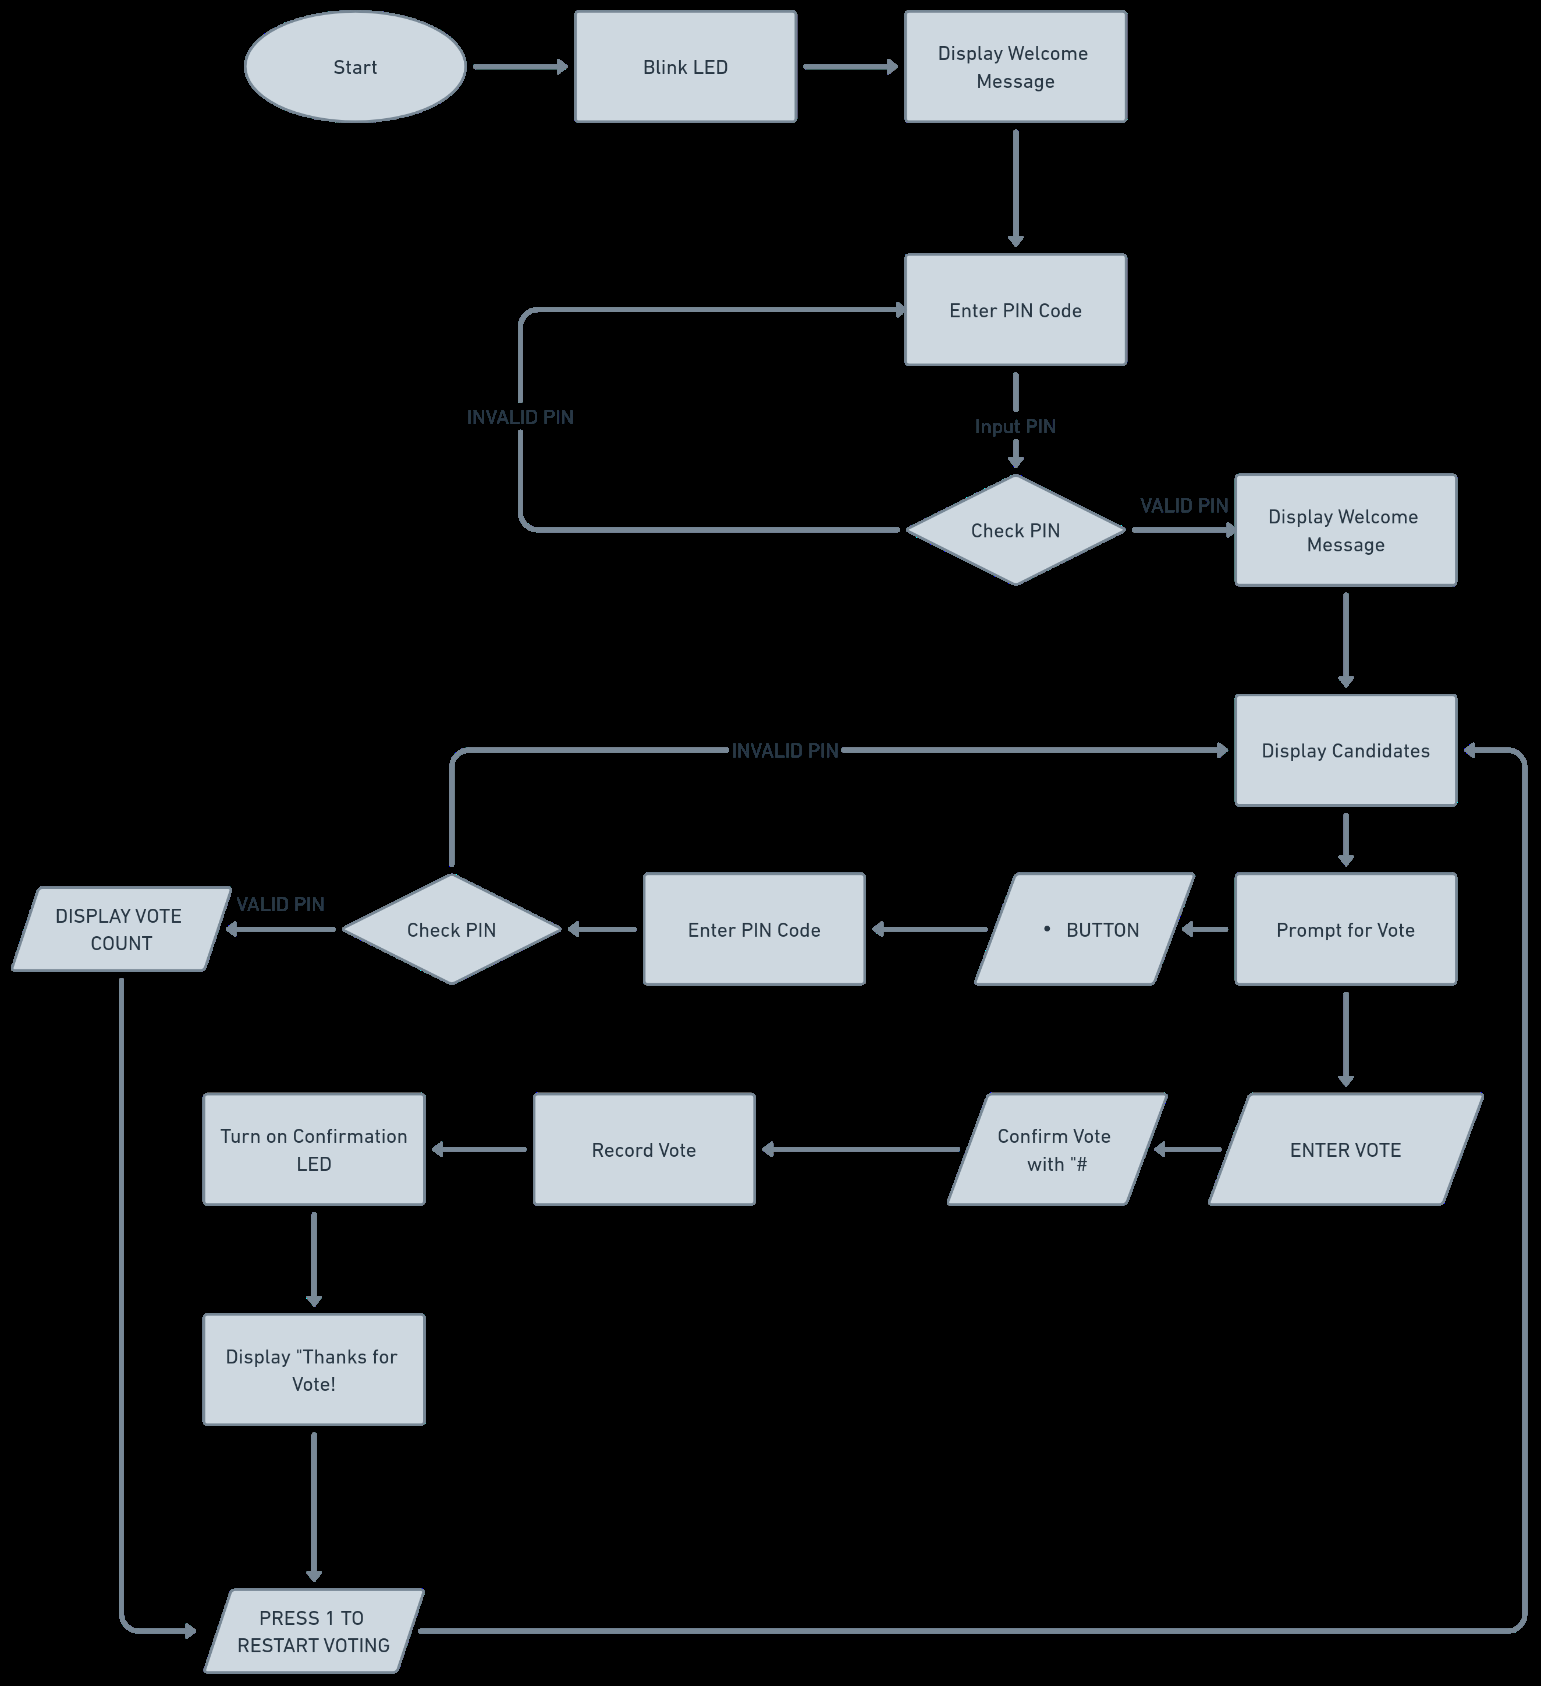
\includegraphics[width=0.85\textwidth]{fig04_voting_system_flowchart.png}
    \caption{Flowchart of the digital voting system.}
    \label{fig:flowchart}
\end{figure}

\section{Pseudo-code}

\begin{lstlisting}[language={}, caption={High-level pseudo-code for the
                   digital voting system}, label={lst:pseudocode}]
Start
    Blink red LED x3
    Keep red LED on
    Display "VOTING SYSTEM"

    loop forever:
        Enter PIN Code  (5 digits, shown as asterisks)
        If PIN invalid:
            Display "INVALID PIN"  -> retry
        Else:
            Display "WELCOME"
            Display Candidates (A / B / C / D)

            Wait for key A-D:
                Display "Vote: X  # to confirm"
            If # pressed:
                Record vote for X
                Blink green LED
                Display "Thanks for Vote!"
                Wait for key 1 to restart

        If * pressed at any time:
            Enter admin PIN
            If valid -> display vote tally (A:n B:n C:n D:n)
            Wait for key 1 to restart
End
\end{lstlisting}

\section{Proteus Simulation Diagram}

\begin{figure}[H]
    \centering
    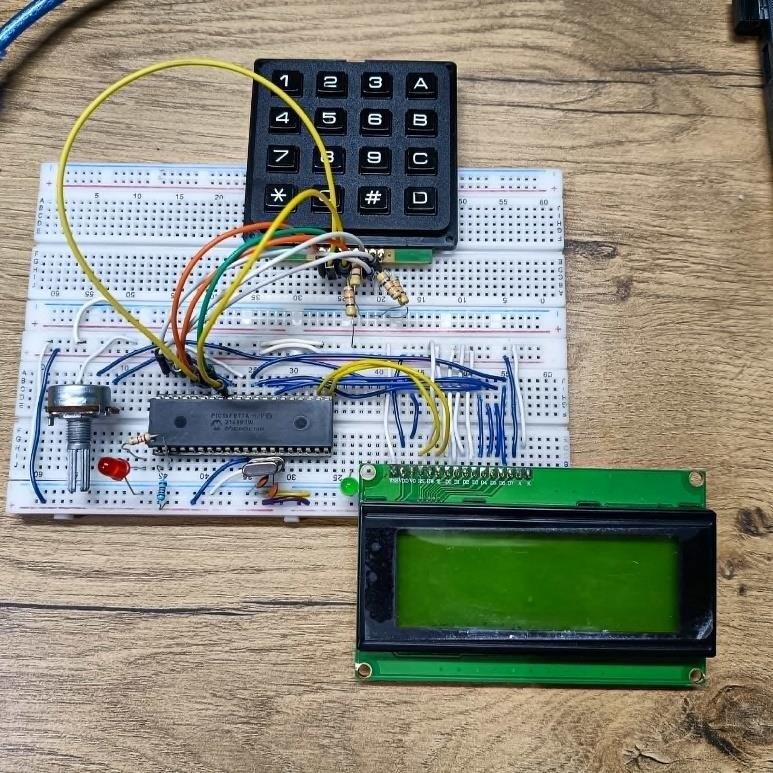
\includegraphics[width=\textwidth]{fig05_simulation_diagram.jpeg}
    \caption{Proteus simulation diagram of the digital voting system.}
    \label{fig:simulation}
\end{figure}

% ============================================================
\chapter{Results and Analysis}
% ============================================================

The digital voting system was tested both in Proteus simulation and on a
physical breadboard. Results are presented below for each operational state,
showing simulation screenshots alongside hardware photographs.

\section{Initial Power-Up}

Upon connecting the PIC16F877A to a \SI{5}{V} supply, the red LED blinks
three times to indicate system start-up, then remains on. The LCD displays
\textit{``Enter PIN Code''}.

\begin{figure}[H]
    \centering
    \begin{minipage}{0.48\textwidth}
        \centering
        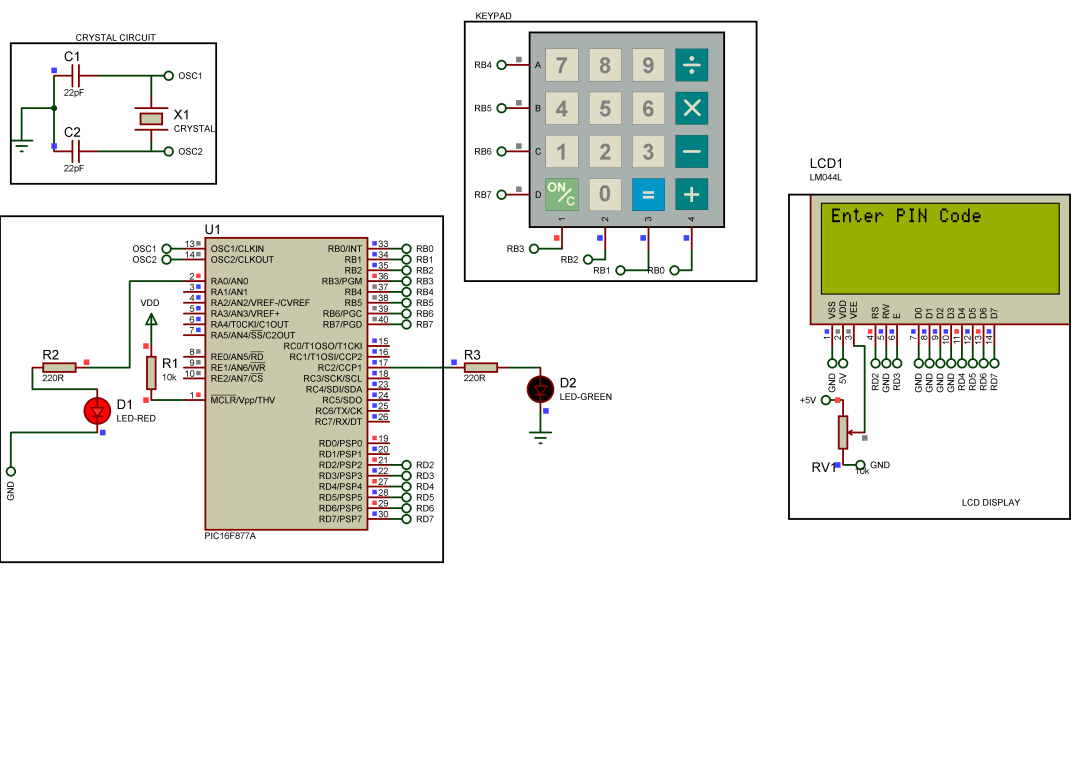
\includegraphics[width=\textwidth]{fig07_initial_state_simulation.png}
        \caption{Initial state --- simulation.}
        \label{fig:init-sim}
    \end{minipage}\hfill
    \begin{minipage}{0.48\textwidth}
        \centering
        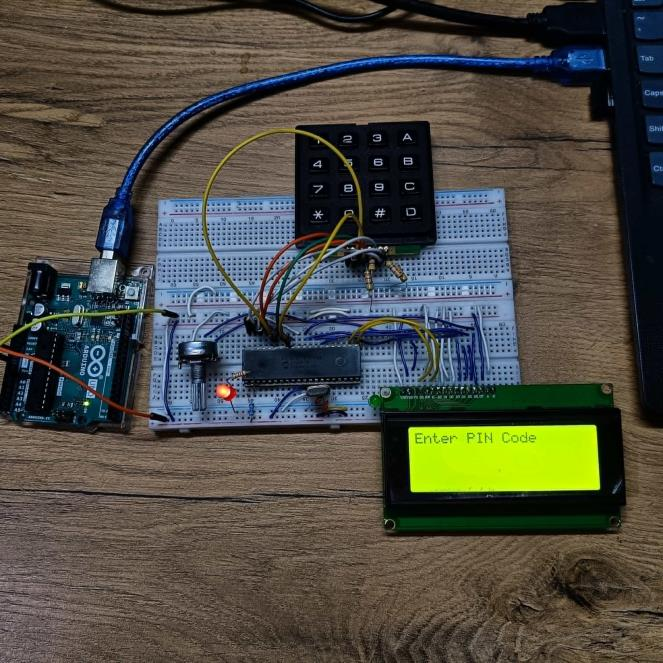
\includegraphics[width=\textwidth]{fig07-1_initial_state_hardware.jpeg}
        \caption{Initial state --- hardware.}
        \label{fig:init-hw}
    \end{minipage}
\end{figure}

\section{Invalid PIN Entry}

When an incorrect PIN is entered, the system displays \textit{``INVALID PIN''}
and returns to the PIN entry prompt. The voting process does not proceed.

\begin{figure}[H]
    \centering
    \begin{minipage}{0.48\textwidth}
        \centering
        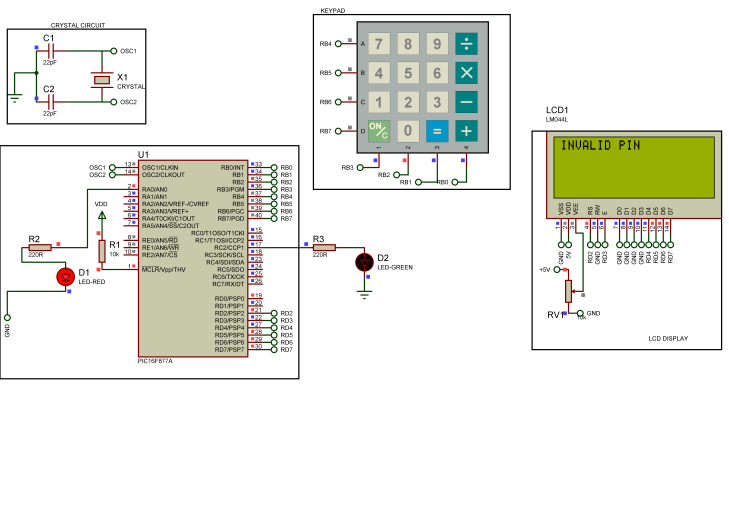
\includegraphics[width=\textwidth]{fig08_invalid_pin_simulation.png}
        \caption{Invalid PIN output --- simulation.}
        \label{fig:invalidpin-sim}
    \end{minipage}\hfill
    \begin{minipage}{0.48\textwidth}
        \centering
        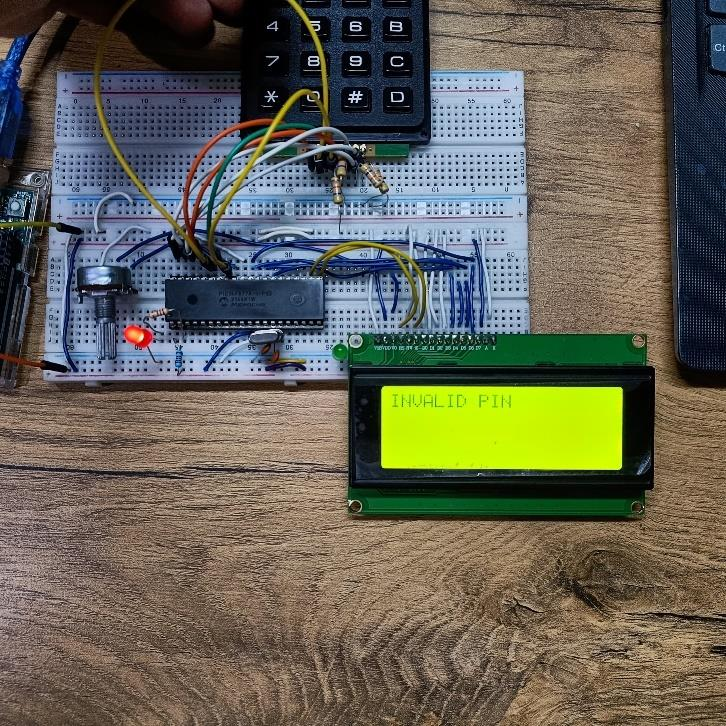
\includegraphics[width=\textwidth]{fig08-1_invalid_pin_hardware.jpeg}
        \caption{Invalid PIN output --- hardware.}
        \label{fig:invalidpin-hw}
    \end{minipage}
\end{figure}

\section{Valid PIN Entry --- Candidate Display}

Upon successful PIN entry the system displays \textit{``WELCOME''} briefly,
then shows all four election candidates on the LCD.

\begin{center}
\texttt{A: KGOTSO \quad B: NIMO}\\
\texttt{C: EKIA \quad\quad D: LOU}
\end{center}

\begin{figure}[H]
    \centering
    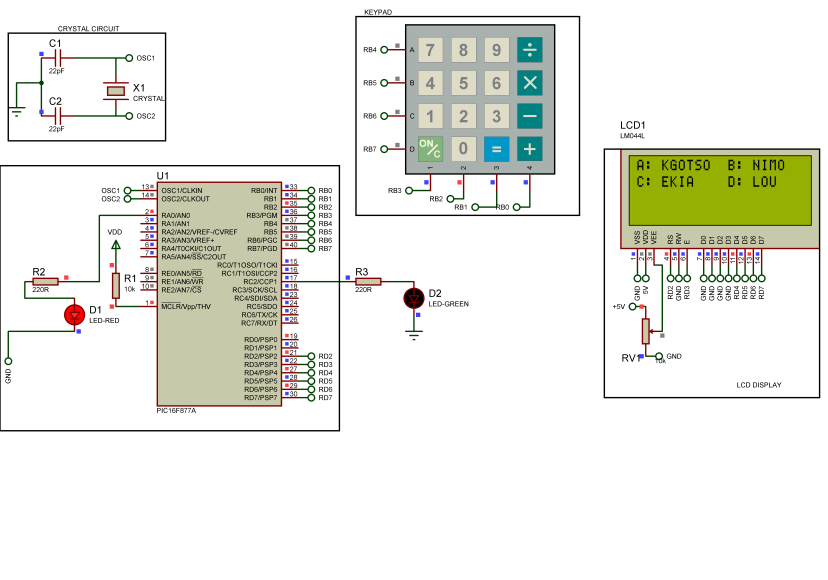
\includegraphics[width=0.58\textwidth]{fig09_valid_pin_simulation.png}
    \caption{Candidate display after valid PIN --- simulation.}
    \label{fig:validpin-sim}
\end{figure}

\section{Waiting for Vote Input}

The LCD prompts \textit{``Vote: / A--D to select''} and waits for the voter
to press a key.

\begin{figure}[H]
    \centering
    \begin{minipage}{0.48\textwidth}
        \centering
        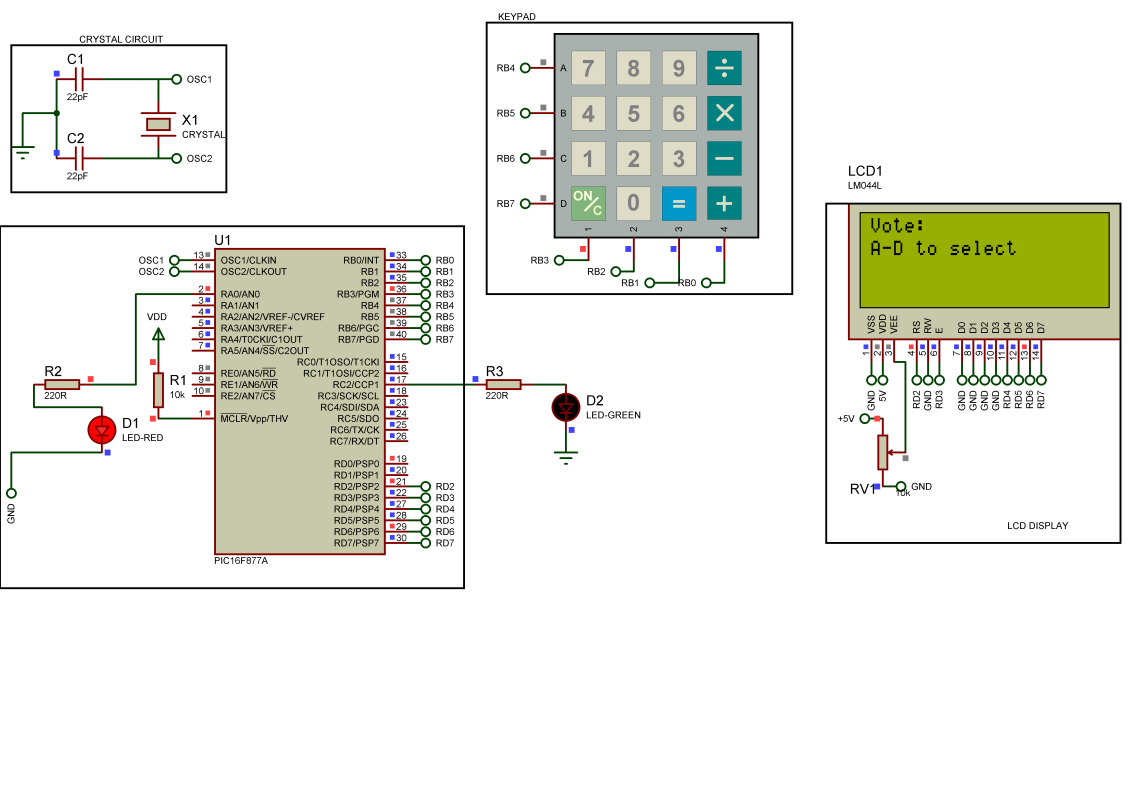
\includegraphics[width=\textwidth]{fig10_waiting_vote_simulation.png}
        \caption{System waiting for vote --- simulation.}
        \label{fig:waitvote-sim}
    \end{minipage}\hfill
    \begin{minipage}{0.48\textwidth}
        \centering
        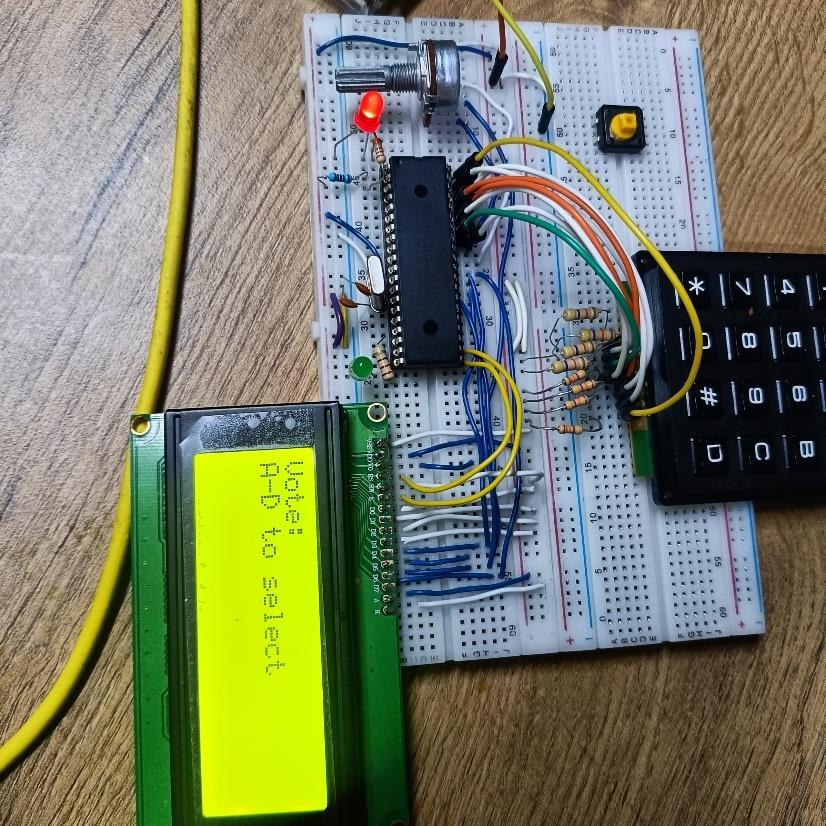
\includegraphics[width=\textwidth]{fig10-1_waiting_vote_hardware.jpeg}
        \caption{System waiting for vote --- hardware.}
        \label{fig:waitvote-hw}
    \end{minipage}
\end{figure}

\section{Vote Confirmation Prompt}

After a candidate key is pressed, the LCD displays \textit{``Vote: X / \# to
confirm''}. The voter must press \texttt{\#} to finalise the vote.

\begin{figure}[H]
    \centering
    \begin{minipage}{0.48\textwidth}
        \centering
        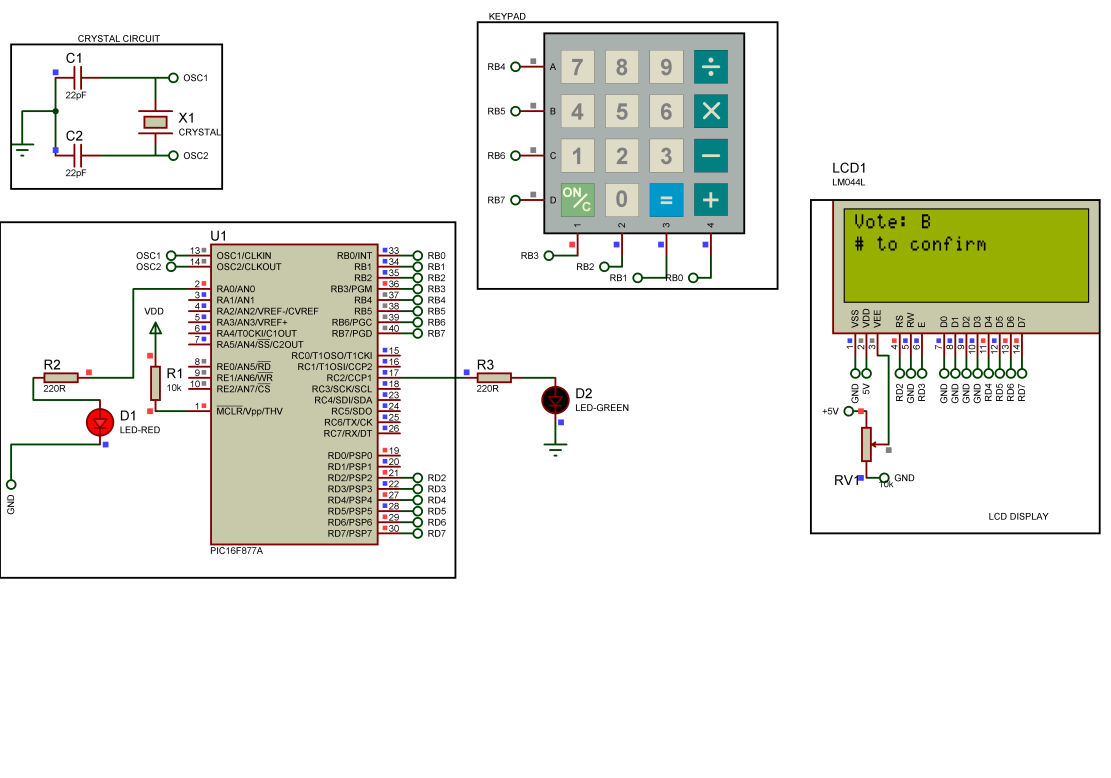
\includegraphics[width=\textwidth]{fig11_confirming_vote_simulation.png}
        \caption{Vote confirmation prompt --- simulation.}
        \label{fig:confirm-sim}
    \end{minipage}\hfill
    \begin{minipage}{0.48\textwidth}
        \centering
        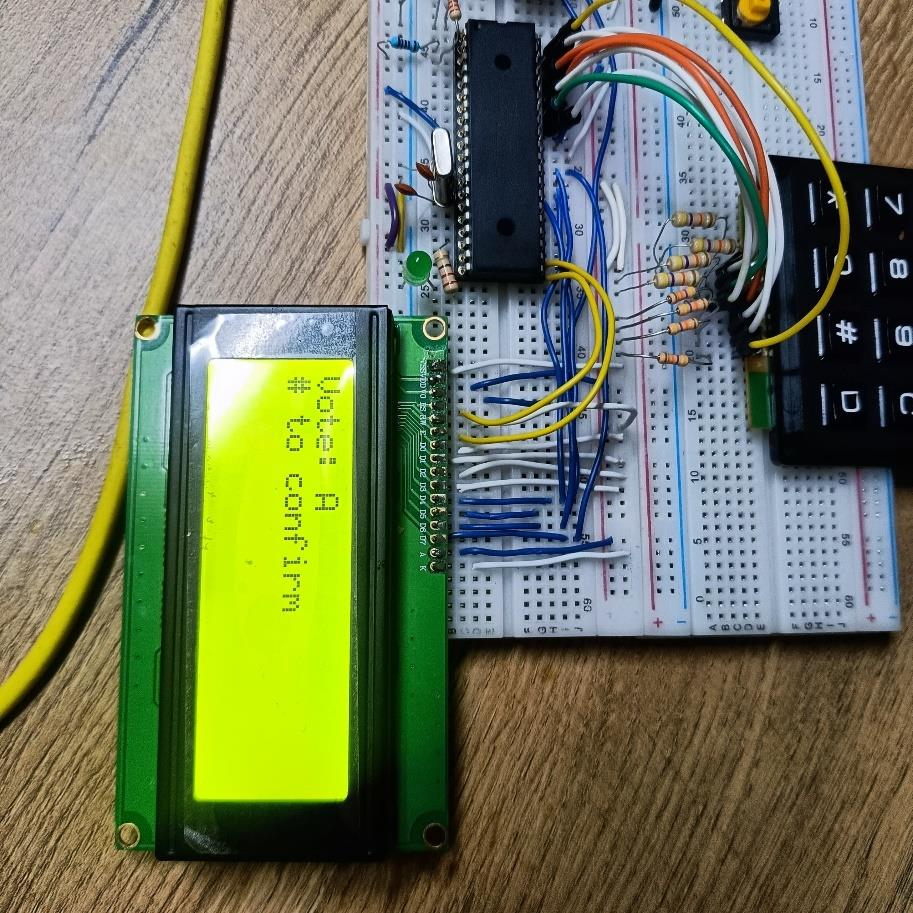
\includegraphics[width=\textwidth]{fig11-1_confirming_vote_hardware.jpeg}
        \caption{Vote confirmation prompt --- hardware.}
        \label{fig:confirm-hw}
    \end{minipage}
\end{figure}

\section{Vote Recorded}

After pressing \texttt{\#}, the vote is recorded, the green LED blinks to
confirm, and the LCD displays \textit{``Thanks for Vote!''}.

\begin{figure}[H]
    \centering
    \begin{minipage}{0.48\textwidth}
        \centering
        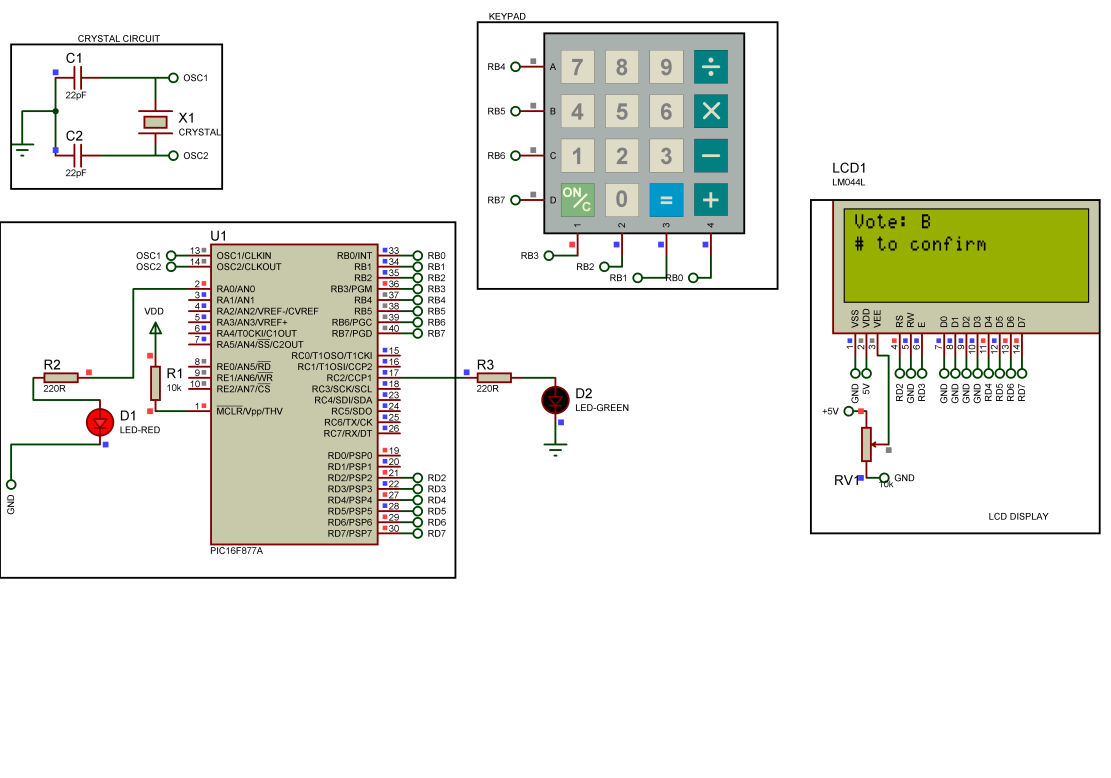
\includegraphics[width=\textwidth]{fig12_confirming_vote2_simulation.png}
        \caption{Vote recorded --- simulation.}
        \label{fig:confirmed-sim}
    \end{minipage}\hfill
    \begin{minipage}{0.48\textwidth}
        \centering
        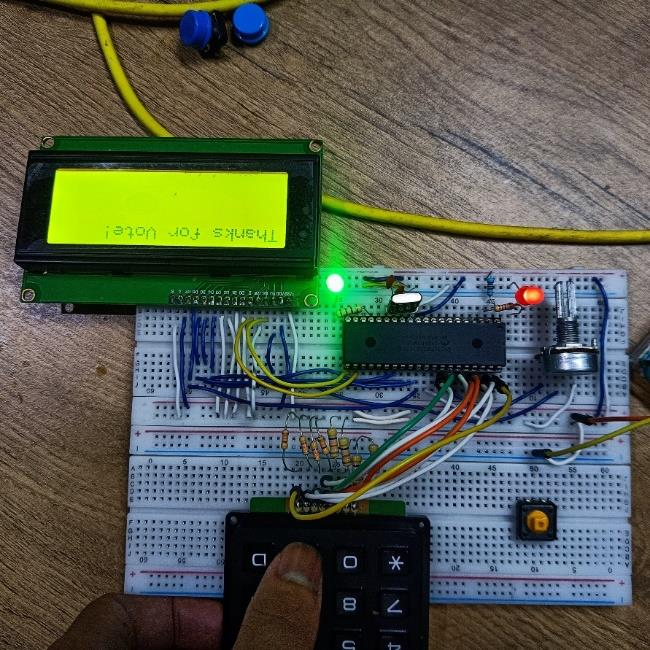
\includegraphics[width=\textwidth]{fig12-1_confirming_vote2_hardware.jpeg}
        \caption{Vote recorded, green LED active --- hardware.}
        \label{fig:confirmed-hw}
    \end{minipage}
\end{figure}

\section{Displaying Vote Statistics}

Pressing \texttt{*} at the voting prompt triggers an admin PIN request. On
correct PIN entry the vote tally is shown: \texttt{A:n\ B:n\ C:n\ D:n}.
An invalid PIN returns \textit{``Invalid PIN''} and exits.

\begin{figure}[H]
    \centering
    \begin{minipage}{0.48\textwidth}
        \centering
        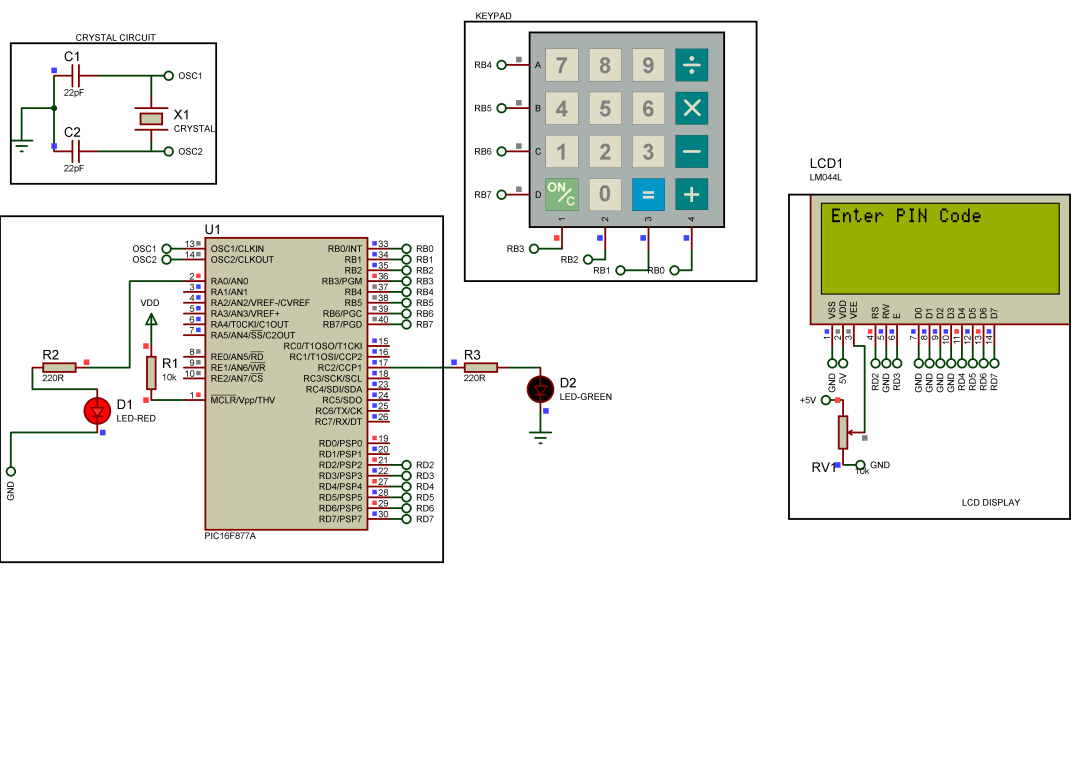
\includegraphics[width=\textwidth]{fig13_vote_tally_pin_simulation.png}
        \caption{Admin PIN request for vote tally --- simulation.}
        \label{fig:tallypin-sim}
    \end{minipage}\hfill
    \begin{minipage}{0.48\textwidth}
        \centering
        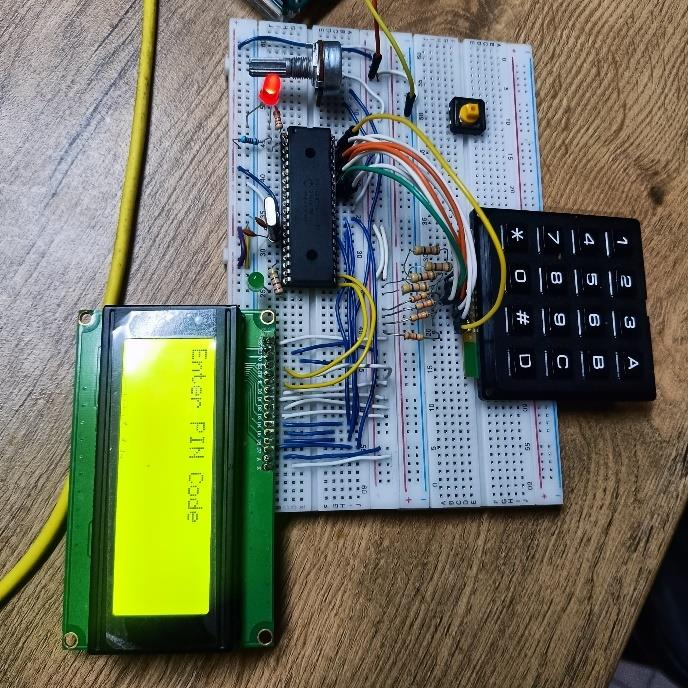
\includegraphics[width=\textwidth]{fig13-1_vote_tally_pin_hardware.jpeg}
        \caption{Admin PIN request for vote tally --- hardware.}
        \label{fig:tallypin-hw}
    \end{minipage}
\end{figure}

\begin{figure}[H]
    \centering
    \begin{minipage}{0.48\textwidth}
        \centering
        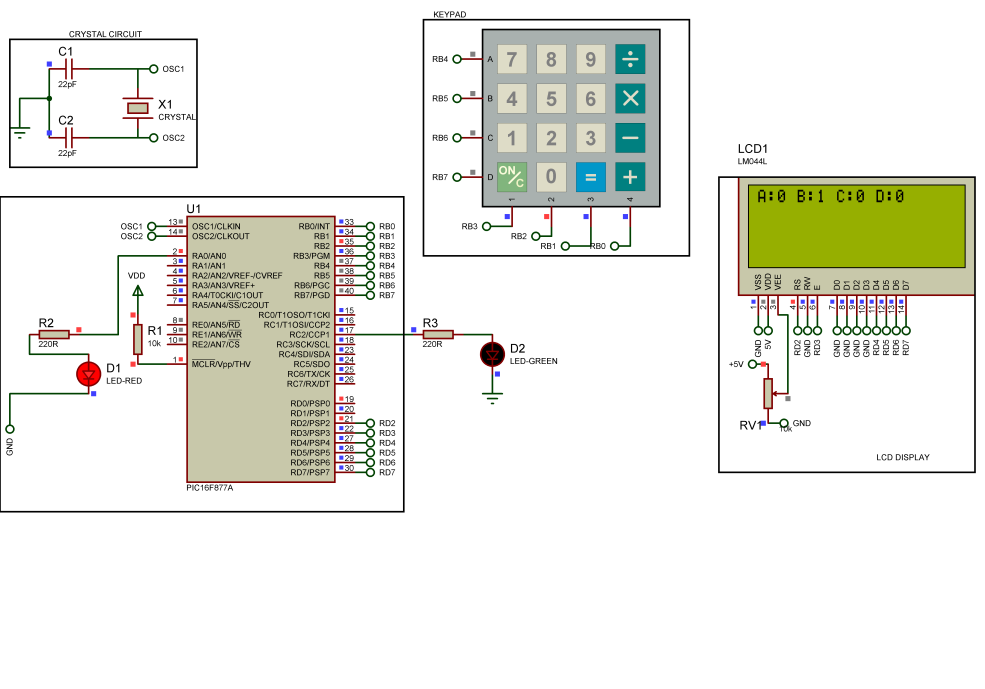
\includegraphics[width=\textwidth]{fig15_voting_statistics_simulation.png}
        \caption{Vote tally display --- simulation.}
        \label{fig:stats-sim}
    \end{minipage}\hfill
    \begin{minipage}{0.48\textwidth}
        \centering
        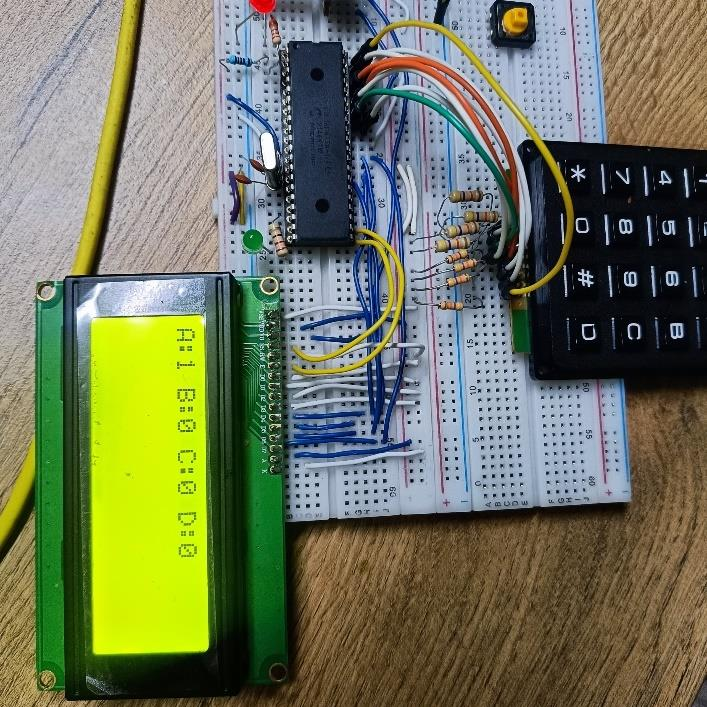
\includegraphics[width=\textwidth]{fig15-1_voting_statistics_hardware.jpeg}
        \caption{Vote tally display --- hardware.}
        \label{fig:stats-hw}
    \end{minipage}
\end{figure}

% ============================================================
\chapter{Discussion}
% ============================================================

The digital voting system was successfully implemented both in Proteus
simulation and on a physical breadboard, meeting all outlined requirements and
demonstrating reliability and user-friendliness.

\section{Security}

PIN-based authentication was implemented at two points: before any voting
session begins, and before vote statistics are displayed. This ensures that
sensitive data remains accessible only to authorised personnel, protecting the
integrity of the election results.

\section{Challenges and Solutions}

The microcontroller, operating at \SI{8}{MHz}, was prone to noise
interference. Prolonged power supply caused some port pins to charge,
resulting in false keypad readings and erroneous characters on the LCD. The
standard approach of grounding only the row pins was insufficient. Grounding
all keypad pin-outs through \SI{47}{\kilo\ohm} pull-down resistors
significantly reduced noise and ensured accurate key detection. This
non-standard configuration proved essential to system stability.

\section{Recommended Future Improvements}

\begin{itemize}
    \item Add decoupling capacitors near the microcontroller power-supply
          pins for additional noise filtering.
    \item Implement software-based debouncing for more robust input
          detection.
    \item Incorporate EEPROM-based non-volatile memory to preserve vote
          counts across power cycles.
    \item Add redundant data storage as an additional security layer.
    \item Expand the candidate list beyond four entries using scrollable
          LCD menus.
\end{itemize}

% ============================================================
\chapter{Conclusion}
% ============================================================

The successful implementation of the digital voting system demonstrates its
potential as a reliable and user-friendly solution for secure electronic
voting. By integrating a \(4 \times 4\) keypad for candidate selection, an
LCD for a clear interface, and LED indicators for visual feedback, the system
provides a seamless voting experience.

Despite initial challenges with noise interference at \SI{8}{MHz} operation,
grounding all keypad pin-outs through \SI{47}{\kilo\ohm} pull-down resistors
proved effective. These solutions highlight the robustness and adaptability of
the design.

The project lays a strong foundation for future advancements in secure digital
voting technologies, with clear pathways for hardware hardening,
software-based debouncing, and persistent storage integration.

%--------------------------------------------------------------
% REFERENCES
%--------------------------------------------------------------
\begin{thebibliography}{9}

\bibitem{geeksforgeeks}
``Microcontroller and its Types,'' \textit{GeeksforGeeks}. [Online].
Available: \url{https://www.geeksforgeeks.org/microcontroller-and-its-types/}.
[Accessed: Nov.\ 15, 2024].

\bibitem{educba}
``Microcontroller Architecture,'' \textit{EDUCBA}. [Online].
Available: \url{https://www.educba.com/microcontroller-architecture/}.
[Accessed: Nov.\ 15, 2024].

\bibitem{microchip}
Microchip Technology Inc., ``PIC16F87XA Data Sheet: 28/40/44-Pin Enhanced
Flash Microcontrollers,'' DS39582E, 2013. [Online].
Available: \url{https://ww1.microchip.com/downloads/en/devicedoc/39582e.pdf}.

\bibitem{raystar}
Raystar Optronics, ``16$\times$4 Character LCD Display Module.'' [Online].
Available:
\url{https://www.raystar-optronics.com/character-lcd-display-module/lcd-16x4.html}.
[Accessed: Nov.\ 1, 2024].

\bibitem{elektronicavoorjou}
Elektronica Voor Jou, ``4$\times$4 Matrix Keypad -- Zwart.'' [Online].
Available:
\url{https://elektronicavoorjou.nl/en/product/4x4-matrix-keypad-zwart/}.
[Accessed: Nov.\ 10, 2024].

\bibitem{lastminuteengineers}
Last Minute Engineers, ``A Beginner's Guide to Keypad Module for Arduino,''
\textit{Last Minute Engineers}. [Online].
Available: \url{https://lastminuteengineers.com/arduino-keypad-tutorial/}.
[Accessed: Nov.\ 10, 2024].

\bibitem{mathangwane}
K.\ Mathangwane, ``Keypad Control System for Microcontroller Project,''
Unpublished Lab Work, Botswana International University of Science and
Technology, Botswana, Nov.\ 2024.

\bibitem{seiphepi}
T.\ Seiphepi, ``Keypad Control System for Microcontroller Project,''
Unpublished Lab Work, Botswana International University of Science and
Technology, Botswana, Nov.\ 2024.

\end{thebibliography}

%--------------------------------------------------------------
% APPENDIX
%--------------------------------------------------------------
\appendix

\chapter{LCD Header File (\texttt{lcd.h})}
\label{app:lcd}

\begin{lstlisting}[caption={lcd.h --- 4-bit LCD driver for PIC16F877A},
                   label={lst:lcdh}]
#ifndef XC_HEADER_TEMPLATE_H
#define XC_HEADER_TEMPLATE_H
#include <xc.h>

void Lcd_Port(char a) {
    D4 = (a & 1) ? 1 : 0;
    D5 = (a & 2) ? 1 : 0;
    D6 = (a & 4) ? 1 : 0;
    D7 = (a & 8) ? 1 : 0;
}
void Lcd_Cmd(char a) { RS = 0; Lcd_Port(a); EN = 1; EN = 0; }
void Lcd_Clear()      { Lcd_Cmd(0); Lcd_Cmd(1); }

void Lcd_Set_Cursor(char a, char b) {
    char temp = (a == 1) ? (0x80 + b - 1) : (0xC0 + b - 1);
    Lcd_Cmd(temp >> 4);
    Lcd_Cmd(temp & 0x0F);
}
void Lcd_Init() {
    Lcd_Port(0x00);
    Lcd_Cmd(0x03); Lcd_Cmd(0x03); Lcd_Cmd(0x03);
    Lcd_Cmd(0x02); Lcd_Cmd(0x02); Lcd_Cmd(0x08);
    Lcd_Cmd(0x00); Lcd_Cmd(0x0C); Lcd_Cmd(0x00); Lcd_Cmd(0x06);
}
void Lcd_Write_Char(char a) {
    char temp = a & 0x0F, y = a & 0xF0;
    RS = 1;
    Lcd_Port(y >> 4); EN = 1; EN = 0;
    Lcd_Port(temp);   EN = 1; EN = 0;
}
void Lcd_Write_String(char *a) {
    for (int i = 0; a[i] != '\0'; i++) Lcd_Write_Char(a[i]);
}
void Lcd_Shift_Right() { Lcd_Cmd(0x01); Lcd_Cmd(0x0C); }
void Lcd_Shift_Left()  { Lcd_Cmd(0x01); Lcd_Cmd(0x08); }

#endif /* XC_HEADER_TEMPLATE_H */
\end{lstlisting}

\chapter{Main Source File (\texttt{D\_VOTING SYSTEM.c})}
\label{app:main}

\begin{lstlisting}[caption={Main source code for the digital voting system},
                   label={lst:main}]
#define _XTAL_FREQ 8000000

#pragma config FOSC  = HS   // High-Speed crystal oscillator
#pragma config WDTE  = OFF  // Watchdog Timer disabled
#pragma config PWRTE = OFF  // Power-up Timer disabled
#pragma config CP    = OFF  // Code Protection off
#pragma config BOREN = OFF  // Brown-out Reset disabled
#pragma config LVP   = OFF  // Low Voltage ICSP disabled
#pragma config CPD   = OFF  // Data EE Memory Code Protection off
#pragma config WRT   = OFF  // Flash Write Protection off

#define RS RD2
#define EN RD3
#define D4 RD4
#define D5 RD5
#define D6 RD6
#define D7 RD7

#include <xc.h>
#include "lcd.h"
#include <stdio.h>
#include <string.h>

int ttlVotesOf_A = 0, ttlVotesOf_B = 0;
int ttlVotesOf_C = 0, ttlVotesOf_D = 0;
char votes[16];
char selectedCandidate = '\0';
const char correctPin[5] = {'8','0','0','8','5'};
char enteredPin[5];
int  pinIndex = 0;

char read_keypad() {
    for (int row = 0; row < 4; row++) {
        PORTB = (1 << row);
        if (PORTBbits.RB4==1) return (row==0)?'A':(row==1)?'3':(row==2)?'2':'1';
        if (PORTBbits.RB5==1) return (row==0)?'B':(row==1)?'6':(row==2)?'5':'4';
        if (PORTBbits.RB6==1) return (row==0)?'C':(row==1)?'9':(row==2)?'8':'7';
        if (PORTBbits.RB7==1) return (row==0)?'D':(row==1)?'#':(row==2)?'0':'*';
    }
    return '\0';
}
void display_candidates() {
    Lcd_Clear();
    Lcd_Set_Cursor(1,1); Lcd_Write_String("A: KGOTSO  B: NIMO");
    Lcd_Set_Cursor(2,1); Lcd_Write_String("C: EKIA    D: LOU");
    __delay_ms(1500);    Lcd_Clear();
}
void enter_pin() {
    Lcd_Clear();
    Lcd_Set_Cursor(1,1); Lcd_Write_String("Enter PIN Code");
    pinIndex = 0;
    while (pinIndex < 5) {
        char key = read_keypad();
        if (key>='0' && key<='9') {
            enteredPin[pinIndex++] = key;
            Lcd_Set_Cursor(2,pinIndex);
            Lcd_Write_String("*");
        }
        __delay_ms(200);
    }
}
void blink_led() {
    for (int i=0; i<3; i++) {
        PORTAbits.RA0=1; __delay_ms(500);
        PORTAbits.RA0=0; __delay_ms(500);
    }
}
void welcome_message() {
    Lcd_Clear(); Lcd_Set_Cursor(1,1);
    Lcd_Write_String(" VOTING SYSTEM ");
    __delay_ms(3000);
}
void wait_for_restart() {
    Lcd_Clear();
    Lcd_Set_Cursor(1,1); Lcd_Write_String("Press 1 to");
    Lcd_Set_Cursor(2,1); Lcd_Write_String("Restart Voting");
    while (1) {
        char key = read_keypad();
        if (key=='1') { welcome_message(); break; }
        __delay_ms(200);
    }
}
void main(void) {
    TRISA=0x00; TRISB=0xF0; TRISD=0x00; TRISC=0x00;
    PORTA=0x00; PORTB=0x00; PORTC=0x00;
    blink_led();
    PORTAbits.RA0=1;
    Lcd_Init();
    welcome_message();
    while (1) {
        int pinCorrect=0;
        while (!pinCorrect) {
            enter_pin();
            if (memcmp(enteredPin,correctPin,5)==0) {
                Lcd_Clear(); Lcd_Set_Cursor(1,1);
                Lcd_Write_String("WELCOME"); __delay_ms(1000);
                pinCorrect=1;
            } else {
                Lcd_Clear(); Lcd_Set_Cursor(1,1);
                Lcd_Write_String("INVALID PIN"); __delay_ms(1000);
            }
            memset(enteredPin,0,5); pinIndex=0;
        }
        while (1) {
            display_candidates();
            Lcd_Clear();
            Lcd_Set_Cursor(1,1); Lcd_Write_String("Vote: ");
            Lcd_Set_Cursor(2,1); Lcd_Write_String("A-D to select");
            while (1) {
                char key=read_keypad();
                if (key=='A'||key=='B'||key=='C'||key=='D') {
                    selectedCandidate=key;
                    Lcd_Clear(); Lcd_Set_Cursor(1,1);
                    char msg[16];
                    sprintf(msg,"Vote: %c",selectedCandidate);
                    Lcd_Write_String(msg);
                    Lcd_Set_Cursor(2,1); Lcd_Write_String("# to confirm");
                } else if (key=='#') {
                    if (selectedCandidate!='\0') {
                        if      (selectedCandidate=='A') ttlVotesOf_A++;
                        else if (selectedCandidate=='B') ttlVotesOf_B++;
                        else if (selectedCandidate=='C') ttlVotesOf_C++;
                        else if (selectedCandidate=='D') ttlVotesOf_D++;
                        Lcd_Clear(); Lcd_Set_Cursor(1,1);
                        Lcd_Write_String("Thanks for Vote!");
                        PORTCbits.RC2=1; __delay_ms(2000);
                        PORTCbits.RC2=0;
                        wait_for_restart(); break;
                    } else {
                        Lcd_Clear(); Lcd_Set_Cursor(1,1);
                        Lcd_Write_String("Invalid Response");
                        __delay_ms(1000); break;
                    }
                } else if (key=='*') {
                    Lcd_Clear(); Lcd_Set_Cursor(1,1);
                    Lcd_Write_String("Enter Vote PIN");
                    enter_pin();
                    if (memcmp(enteredPin,correctPin,5)==0) {
                        Lcd_Clear(); Lcd_Set_Cursor(1,1);
                        sprintf(votes,"A:%d B:%d C:%d D:%d",
                            ttlVotesOf_A,ttlVotesOf_B,
                            ttlVotesOf_C,ttlVotesOf_D);
                        Lcd_Write_String(votes);
                        __delay_ms(5000);
                        wait_for_restart(); break;
                    } else {
                        Lcd_Clear(); Lcd_Set_Cursor(1,1);
                        Lcd_Write_String("Invalid PIN");
                        __delay_ms(1000); break;
                    }
                    memset(enteredPin,0,5); pinIndex=0;
                } else if (key!='\0') {
                    Lcd_Clear(); Lcd_Set_Cursor(1,1);
                    Lcd_Write_String("Invalid Response");
                    __delay_ms(1000); break;
                }
                __delay_ms(200);
            }
        }
    }
}
\end{lstlisting}

\end{document}
